% !TeX program = xelatex
%\documentclass[9pt]{beamer}
\documentclass[9pt, aspectratio=169]{beamer}
\usepackage{xcolor}
\definecolor{orange}{HTML}{FF1053}
\definecolor{lightgray}{HTML}{CCCCCC}
\definecolor{red}{HTML}{AC454A}
\definecolor{brown}{HTML}{EAD296}
\definecolor{darkgrey}{HTML}{313630}
\definecolor{cornflower}{HTML}{247BA0}
\definecolor{sienna}{HTML}{6C464F}
\usefonttheme{professionalfonts} % using non standard fonts for beamer
\usefonttheme{serif} % default family is serif
\usepackage{fontspec}
\usepackage{setspace}
\usepackage{bm}
\usepackage{natbib}
\usepackage{animate}
\usepackage{graphicx}
\usepackage{algorithm2e}
\usepackage{amsmath, amssymb}
%\usepackage[T1]{fontenc}
\newcommand{\diff}{\,\mathrm{d}}
\bibliographystyle{abbrv}
%\setmainfont{Liberation Serif}
%\setmainfont{Liberation Serif}
\setmainfont{Comfortaa}
%\usepackage[T1]{fontenc}

\setbeamercolor{frametitle}{bg=orange,fg=white}
\setbeamercolor{author in head/foot}{bg=orange,fg=white}

%\setbeamerfont{page number}{size=\Huge}

%\setbeamertemplate{itemize itemjpegs}[circle]
\useinnertheme{circles}
\setbeamercolor{palette primary}{bg=orange,fg=white}
%\setbeamercolor{palette secondary}{bg=red,fg=white}
\setbeamertemplate{itemize item}{\color{darkgrey}$\circ$}
\setbeamercolor{structure}{fg=darkgrey} % itemize, enumerate, etc

%\setbeamercolor{section in head/foot}{bg=red}
\setbeamercolor{title}{fg=orange} %, bg=brown
\setbeamercolor{author}{fg=darkgrey}
\setbeamercolor{institute}{fg=darkgrey}
\setbeamercolor{date}{fg=darkgrey}
%\setbeamercolor{normal text}{fg=darkgrey}
\makeatletter
\setbeamertemplate{headline}{%
	\usebeamercolor[bg]{frametitle}\rule{\textwidth}{1cm}
}
\setbeamerfont{title}{size=\LARGE}
\setbeamerfont{institute}{size=\normalsize}
\renewcommand*{\bibfont}{\scriptsize}


\setbeamertemplate{frametitle}{%
	\vskip-1cm%
	\begin{minipage}[c][\headheight][c]{\textwidth}%
		\usebeamerfont{frametitle}
		\strut\insertframetitle\par
		{%
			\ifx\insertframesubtitle\@empty%
			\else%
			{\usebeamerfont{framesubtitle}\usebeamercolor[fg]{framesubtitle}\strut\insertframesubtitle\par}%
			\fi
		}%      
		\vspace*{0.05cm}
	\end{minipage}%
	\vskip-0.1em
}
%\setbeamertemplate{footline}{%
%	\leavevmode%
%	\hbox{\begin{beamercolorbox}[wd=\paperwidth,ht=4.5ex,dp=3.125ex]{author in head/foot}%
%			\usebeamerfont{author in head/foot} bar
%	\end{beamercolorbox}}%
%	\vskip0pt%
%}
\makeatother


\title{Simulation-based Inference \\
	\small Learning a Posterior by Inverting Simulators}
\author{Talk by Stefan Wezel}
\institute{mlcolab @ Tübingen University}
\date{\today}


%\setbeamertemplate{sidebar right}{}
%\setbeamertemplate{footline}{%
%	\hfill\usebeamertemplate***{navigation symbols}
%	\hspace{1cm}\insertframenumber{}}
\setbeamerfont{page number in head/foot}{size=\small}
    \setbeamertemplate{footline}{%
	\raisebox{5pt}{\makebox[\paperwidth]{\hfill\makebox[10pt]{\scriptsize\insertframenumber}}}}
\setbeamertemplate{navigation symbols}{}
%\onehalfspacing
\setstretch{1.3}
\begin{document}
	

\setbeamercolor{background canvas}{bg=white}
\setbeamercolor{normal text}{fg=darkgrey}
\usebeamercolor[fg]{normal text}
\begin{frame}[plain]
	\titlepage
\end{frame} 



\setbeamercolor{background canvas}{bg=white}
\setbeamercolor{normal text}{fg=darkgrey}
\usebeamercolor[fg]{normal text}
\setbeamertemplate{itemize item}{\color{darkgrey}$\circ$}
\begin{frame}
\frametitle{Overview}
\framesubtitle{}
\begin{itemize}
	\item Problem Setting %(as this is rather unfamiliar to ML researchers)
	\item Traditional Approaches and their Issues
	\item Using Neural Networks to alleviate them
	\item SBI in the Wild
%	\item Outlook %(and some advertisement)
\end{itemize}
\end{frame} 






\begin{frame}
\frametitle{What and Why?}
\framesubtitle{What is a simulator?}
\begin{itemize}
	\item Inverting simulators?% - so first let's find out what a simulator is
	\item What is a simulator? % in context of this presentation
	\begin{itemize}
		\item Forward, generative model with parameters and stochasticity
		\item Produces observations
		\item In context of this talk computer program, but can be electrical circuit (Hodgkin–Huxley model)
	\end{itemize}
	\item Used by scientists to model empirically observed data
	\item In particle physics, population genetics, epidemiology
	\item Encode knowledge about systems
\end{itemize}
\end{frame} 



\begin{frame}
\frametitle{What and Why?}
\framesubtitle{An Example}
	\begin{figure}
	\includegraphics[width=.85\linewidth]{figures/lhc1.pdf}
\end{figure}
\tiny Figure derived from \textit{cern.ch, Achintya Rao and Tom McCauley, sciencealert.com}
\end{frame}
\begin{frame}
\frametitle{What and Why?}
\framesubtitle{An Example}
\begin{figure}
	\includegraphics[width=.85\linewidth]{figures/lhc2.pdf}
\end{figure}
\tiny Figure derived from \textit{cern.ch, Achintya Rao and Tom McCauley, sciencealert.com}
\end{frame}
\begin{frame}
\frametitle{What and Why?}
\framesubtitle{An Example}
\begin{figure}
\includegraphics[width=.85\linewidth]{figures/lhc3.pdf}
\end{figure}
\tiny Figure derived from \textit{cern.ch, Achintya Rao and Tom McCauley, sciencealert.com}
\end{frame} \begin{frame}
\frametitle{What and Why?}
\framesubtitle{An Example}
\begin{figure}
\includegraphics[width=.85\linewidth]{figures/lhc4.pdf}
\end{figure}
\tiny Figure derived from \textit{cern.ch, Achintya Rao and Tom McCauley, sciencealert.com}
\end{frame} \begin{frame}
\frametitle{What and Why?}
\framesubtitle{An Example}
\begin{figure}
\includegraphics[width=.85\linewidth]{figures/lhc5.pdf}
\end{figure}
\tiny Figure derived from \textit{cern.ch, Achintya Rao and Tom McCauley, sciencealert.com}
\end{frame} \begin{frame}
\frametitle{What and Why?}
\framesubtitle{An Example}
\begin{figure}
\includegraphics[width=.85\linewidth]{figures/lhc6.pdf}
\end{figure}
\tiny Figure derived from \textit{cern.ch, Achintya Rao and Tom McCauley, sciencealert.com}
\end{frame} \begin{frame}
\frametitle{What and Why?}
\framesubtitle{An Example}
\begin{figure}
\includegraphics[width=.85\linewidth]{figures/lhc7.pdf}
\end{figure}
\tiny Figure derived from \textit{cern.ch, Achintya Rao and Tom McCauley, sciencealert.com}
\end{frame} 



\begin{frame}
\frametitle{What and Why?}
\framesubtitle{Formalizing our Example}
\begin{itemize}
%	\item Before we go into SBI, let's take a minute to formalize our setting
	\item Simulator has parameters $\theta$, nuisance parameter $z$
	\item Produces data $x$
	\begin{itemize}
		\item Implicitly defines $p(x,z\mid\theta)$ %(it yields samples from this distribution)
	\end{itemize}
	\item Given (real) observation $x_0$, we are interested in parameters that produced it
%	\begin{align}\\
	\begin{align}
p(\theta\mid x=x_0) = \frac{p(x\mid\theta)p(\theta)}{p(x)} = \frac{\overbrace{\int p(x,z\mid\theta)\diff z}^{\text{intractable}} p(\theta)}{\int p(x\mid\theta)p(\theta) \diff \theta}
\end{align}
\item Typical problem setting of scientists across domains
\begin{itemize}
			\item Sophisticated forward model that encapsulates prior knowledge
	\item Inference means: What were parameters that produced observation?
\end{itemize}
\item To find $\theta$, invert simulator
%	p(\theta\mid x=x_0) = \frac{p(x\mid\theta)p(\theta)}{p(x)} = \frac{\overbrace{\int p(x,z\mid\theta)dz}^{intractable} p(\theta)}{\underbrace{\int p(x\mid\theta)p(\theta)\theta}_{intractable}},
%	\end{align}
%	\begin{itemize}
%		\item $p(\theta\mid x_0)$ -> posterior over parameters
%		\item In simple cases, we could apply Bayes' rule and compute it analytically
%		\item What is simple? If we know Likelihood
%		\item But often we would not
%	\end{itemize}
%\item $q_{\phi}(\theta\mid x)=\Sigma_k \alpha_k\mathcal{N}(\theta\midm_{k}, S_{k}) \sim$
\end{itemize}
\end{frame} 



%\begin{frame}
%\frametitle{What and Why?}
%\framesubtitle{Simulation-based Inference to the rescue}
%\begin{itemize}
%		\item Typical problem setting of scientists across domains
%	\begin{itemize}
%		\item Sophisticated forward model that encapsulates prior knowledge
%		\item Inference means: What were parameters that produced observation?
%	\end{itemize}
%	\item SBI tries to solve this problem
%%	\item It tries to invert simulator
%	\item By inverting simulator
%\end{itemize}
%\end{frame} 




%\begin{frame}
%\frametitle{When is this useful?}
%\framesubtitle{SBI at LHC}
%\begin{itemize}
%	\item Simulator of standard model of particle physics
%	\item many parameters
%	\begin{itemize}
%		\item parameters $\theta$
%		\item nuisance parameters $z$ (particle momenta, splitting, detector interaction, ..)
%	\end{itemize}
%	\item that produce observation $x$
%	\item likelihood $\int p(x,z\mid\theta)dz$ intractable
%\end{itemize}
%		\begin{figure}
%%	\flushleft
%	\includegraphics[width=.6\linewidth]{figures/lhc.jpg}
%\end{figure}
%\end{frame} 
%



\begin{frame}
\frametitle{Simulation-based Inference}
\framesubtitle{Traditional Approach}
\begin{itemize}
	\item Broader term: Approximate Bayesian Computation (ABC)
		\item Rejection ABC
		\begin{itemize}
				\item Change $\theta$ until something $\epsilon$-close to $x_0$ is produced
				\item Inefficient for small $\epsilon$
				\item No actual posterior but only point estimate
				\item Approximates $p(\theta\mid\mid\mid x-x_0 \mid\mid < \epsilon)$
		\end{itemize}
	\item Some improvements
	\begin{itemize}
		\item Sampling ABC (perturb matched parameters) \cite{marjoram2003markov}
		\item Sequential ABC (importance sampling) \cite{beaumont2009adaptive,bonassi2015sequential}
	\end{itemize}
%		\item But gives only point estimates, not full posterior
	\item Point-estimate to posterior over parameters for $\epsilon$-ball around observation
%	\item Not actual posterior
	
%	Found parameters not from actual posterior but from $\epsilon$-approximation to it
%		\item within $\epsilon$
%	\item Some improvements are MCMC ABC and Sequential ABC but they only improve sample efficiency but still produce merely point estimate	
\end{itemize}
\end{frame} 



\begin{frame}
\frametitle{Simulation-based Inference}
\framesubtitle{Predicting Parameter Posterior}
\begin{itemize}
	\item Papamakarios and Murray \cite{papamakarios2016fast} learn approximation to actual posterior
	\item Use simulator to create training set
	\begin{itemize}
		\item $\lbrace x_j, \theta_j \rbrace_{j \in N}$
	\end{itemize}
	\item Train neural network to predict parameters of posterior over $\theta$s 
\end{itemize}
\end{frame} 


%%%%%%%%%% posterior algo
%\begin{frame}
%\frametitle{Simulation-based Inference}
%\framesubtitle{Predicting Parameter Posterior}
%\begin{algorithm}[H]
%%	\tcp{Create training set}
%	\color{orange}\For{$n=1..N$}{
%		sample $\theta_n \sim \tilde{p}(\theta)$ \\
%		sample $x_n \sim p(x\mid\theta_n)$ \\
%	}
%%	\tcp{Find variational posterior over parameters}
%	\color{black}train $q_{\phi}(\theta\mid x)$ on $\lbrace x_n,\theta_n \rbrace$\\
%%	\tcp{Find posterior over parameters for given observation}
%%	$\hat{p}(\theta\mid x=x_0) \leftarrow \frac{p(\theta)}{\tilde{p}(c)}q_{\phi}(\theta\mid x)$
%	sample $\theta \sim q(\theta \mid x=x_0)$
%\end{algorithm}
%\vspace{35pt}
%\tiny Pseudocode derived from \cite{papamakarios2016fast}
%\end{frame}
%\begin{frame}
%\frametitle{Simulation-based Inference}
%\framesubtitle{Predicting Parameter Posterior}
%\begin{algorithm}[H]
%	%	\tcp{Create training set}
%	\For{$n=1..N$}{
%		sample $\theta_n \sim \tilde{p}(\theta)$ \\
%		sample $x_n \sim p(x\mid\theta_n)$ \\
%	}
%	%	\tcp{Find variational posterior over parameters}
%	\color{orange}train $q_{\phi}(\theta\mid x)$ on $\lbrace x_n,\theta_n \rbrace\;$\color{black} (More in a second)\\
%	%	\tcp{Find posterior over parameters for given observation}
%%	\color{black}$\hat{p}(\theta\mid x=x_0) \leftarrow \frac{p(\theta)}{\tilde{p}(c)}q_{\phi}(\theta\mid x)$
%	sample $\theta \sim q(\theta \mid x=x_0)$
%\end{algorithm}
%\vspace{35pt}
%\tiny Pseudocode derived from \cite{papamakarios2016fast}
%\end{frame} 
%\begin{frame}
%\frametitle{Simulation-based Inference}
%\framesubtitle{Predicting Parameter Posterior}
%\begin{algorithm}[H]
%	%	\tcp{Create training set}
%	\For{$n=1..N$}{
%		sample $\theta_n \sim \tilde{p}(\theta)$ \\
%		sample $x_n \sim p(x\mid\theta_n)$ \\
%	}
%	%	\tcp{Find variational posterior over parameters}
%	\color{black}train $q_{\phi}(\theta\mid x)$ on $\lbrace x_n,\theta_n \rbrace$\\
%	%	\tcp{Find posterior over parameters for given observation}
%%	\color{orange}$\hat{p}(\theta\mid x=x_0) \leftarrow \frac{p(\theta)}{\tilde{p}(c)}q_{\phi}(\theta\mid x)$
%\color{orange}	sample $\theta \sim q(\theta \mid x=x_0)$
%\end{algorithm}
%\vspace{35pt}
%\tiny Pseudocode derived from \cite{papamakarios2016fast}
%\end{frame} 


%%%%%%%%% sbi visualizations
\begin{frame}
\frametitle{Learning a Posterior}
\framesubtitle{from Simulations}
\begin{figure}
	\includegraphics[width=1\linewidth]{figures/sbi1.pdf}
\end{figure}
\end{frame} 
\begin{frame}
\frametitle{Learning a Posterior}
\framesubtitle{from Simulations}
\begin{figure}
	\includegraphics[width=1\linewidth]{figures/sbi2.pdf}
\end{figure}
\end{frame} \begin{frame}
\frametitle{Learning a Posterior}
\framesubtitle{from Simulations}
\begin{figure}
\includegraphics[width=1\linewidth]{figures/sbi3.pdf}
\end{figure}
\end{frame} \begin{frame}
\frametitle{Learning a Posterior}
\framesubtitle{from Simulations}
\begin{figure}
\includegraphics[width=1\linewidth]{figures/sbi4.pdf}
\end{figure}
\end{frame} \begin{frame}
\frametitle{Learning a Posterior}
\framesubtitle{from Simulations}
\begin{figure}
\includegraphics[width=1\linewidth]{figures/sbi5.pdf}
\end{figure}
\end{frame} \begin{frame}
\frametitle{Learning a Posterior}
\framesubtitle{from Simulations}
\begin{figure}
\includegraphics[width=1\linewidth]{figures/sbi6.pdf}
\end{figure}
\end{frame}




\begin{frame}
\frametitle{Updating the Prior}
\framesubtitle{With the Posterior}
\begin{itemize}
	\item What if we only care about single observation?
%	\item Lueckmann et al. propose faster version
	\item Iteratively replace prior with posterior
	\item Faster convergence
\end{itemize}
\begin{figure}
	\includegraphics[width=.8\linewidth]{figures/sbiproposalprior.pdf}
\end{figure}
\end{frame} 



%%%%%%%%%%%%% prior algo
%%%%%%%%%sbi algo
\begin{frame}
\frametitle{Updating the Prior}
\framesubtitle{With the Posterior}
\begin{algorithm}[H]
%	\tcp{Initial proposal prior}
	$\color{orange}\tilde{p}(\theta) \leftarrow p(\theta)$\\
%	\tcp{Create training set}
	\Repeat{$\tilde{p}(\theta)$ has converged}{
		\For{$n=1..N$}{
			sample $\theta_n \sim \tilde{p}(\theta)$ \\
			sample $x_n \sim p(x\mid\theta_n)$ \\
		}
		train $q_{\phi}(\theta\mid x)$ on $\lbrace x_n, \theta_n \rbrace$\\
%		$\hat{p}(\theta\mid x=x_0) \leftarrow \frac{p(\theta)}{\tilde{p}(c)}q_{\phi}(\theta\mid x)$
%sample $\theta \sim q(\theta \mid x=x_0)$
$\tilde{p}(\theta) \leftarrow q_{\phi}(\theta\mid x)$
	}
\end{algorithm}
\vspace{35pt}
\tiny Pseudocode derived from \cite{papamakarios2016fast}
\end{frame} 
\begin{frame}
\frametitle{Updating the Prior}
\framesubtitle{With the Posterior}
\begin{algorithm}[H]
	$\tilde{p}(\theta) \leftarrow p(\theta)$\\
	\Repeat{$\tilde{p}(\theta)$ has converged}{
		\color{orange}\For{$n=1..N$}{
			sample $\theta_n \sim \tilde{p}(\theta)$ \\
			sample $x_n \sim p(x\mid\theta_n)$ \\
		}

		train $q_{\phi}(\theta\mid x)$ on $\lbrace x_n, \theta_n \rbrace$\\
%			\color{black}$\hat{p}(\theta\mid x=x_0) \leftarrow \frac{p(\theta)}{\tilde{p}(c)}q_{\phi}(\theta\mid x)$
\color{black}$\tilde{p}(\theta) \leftarrow q_{\phi}(\theta\mid x)$
	}
\end{algorithm}
\vspace{35pt}
\tiny Pseudocode derived from \cite{papamakarios2016fast}
\end{frame} 

\begin{frame}
\frametitle{Updating the Prior}
\framesubtitle{With the Posterior}
\begin{algorithm}[H]
	%	\tcp{Initial proposal prior}
	$\tilde{p}(\theta) \leftarrow p(\theta)$\\
	%	\tcp{Create training set}
	\Repeat{$\tilde{p}(\theta)$ has converged}{
		\For{$n=1..N$}{
			sample $\theta_n \sim \tilde{p}(\theta)$ \\
			sample $x_n \sim p(x\mid\theta_n)$ \\
		}
		train $q_{\phi}(\theta\mid x)$ on $\lbrace x_n, \theta_n \rbrace$\\
%		\color{orange}$\hat{p}(\theta\mid x=x_0) \leftarrow \frac{p(\theta)}{\tilde{p}(c)}q_{\phi}(\theta\mid x)$
\color{orange}$\tilde{p}(\theta) \leftarrow q_{\phi}(\theta\mid x)$}
\end{algorithm}
\vspace{35pt}
\tiny Pseudocode derived from \cite{papamakarios2016fast}
\end{frame} 
\begin{frame}
\frametitle{Updating the Prior}
\framesubtitle{With the Posterior}
\begin{algorithm}[H]
	%	\tcp{Initial proposal prior}
	$\tilde{p}(\theta) \leftarrow p(\theta)$\\
	%	\tcp{Create training set}
	\Repeat{\color{orange}$\tilde{p}(\theta)$ has converged}{
		\For{$n=1..N$}{
			sample $\theta_n \sim \tilde{p}(\theta)$ \\
			sample $x_n \sim p(x\mid\theta_n)$ \\
		}
		train $q_{\phi}(\theta\mid x)$ on $\lbrace x_n, \theta_n \rbrace$\\
%		$\hat{p}(\theta\mid x=x_0) \leftarrow \frac{p(\theta)}{\tilde{p}(c)}q_{\phi}(\theta\mid x)$
	$\tilde{p}(\theta) \leftarrow q_{\phi}(\theta\mid x)$}
\end{algorithm}
\vspace{35pt}
\tiny Pseudocode derived from \cite{papamakarios2016fast}
\end{frame} 



%\begin{frame}
%\frametitle{Learning a Posterior}
%\framesubtitle{Bayesian Neural Nets to the Rescue}
%\begin{itemize}
%	\item Create $n$ training samples
%	\item learn posterior over parameters by parametrizing GMM with DNN
%\end{itemize}
%\end{frame}
\begin{frame}
\frametitle{Applying SBI}
\framesubtitle{to Hodgkin–Huxley}
\begin{itemize}
	\item Lueckmann et al. \cite{lueckmann2017flexible} apply SBI to neuroscience setting
	\begin{itemize}
		\item Diverging simulations
%		\item Corrupt data
		\item Summary statistics challenging
	\end{itemize}
	\item They propose
	\begin{itemize}
			\item Train classifier to predict whether parameters fail
%		\item Handle bad simulations to improve convergence (i.e. diverging firing rate)
%		\begin{itemize}
%		\end{itemize}
		\item Extract features with RNN
					\item Posterior over network weights%, that can be used to init network in next iteration
	\end{itemize}
		\item Apply Hodgkin-Huxley model \cite{hodgkin1952quantitative} 
\begin{itemize}
	\item Numerical simulators available (NEURON software \cite{carnevale2006neuron})
	\item Dynamics of neuron's membrane
	\item Parameters (concentration of sodium, potassium, ...)
\end{itemize}
\end{itemize}
\end{frame}  
%\begin{frame}
%\frametitle{Refining SBI}
%\framesubtitle{Lueckman et al}
%\begin{itemize}
%%	\item Include importance reweighting in loss
%%	\begin{itemize}
%%		\item No analytical step necessary
%%		\item Enables complex proposal priors
%%	\end{itemize}
%
%\end{itemize}
%\end{frame} 


%%%%%%%%%%%% Application to Hodgkin-Huxley

\begin{frame}
\frametitle{Applying SBI}
\framesubtitle{Results}
\begin{figure}
	\includegraphics[width=.8\linewidth]{figures/sbineuron1.pdf}
\end{figure}
\vspace{50pt}
\tiny Figure derived from \cite{lueckmann2017flexible}
\end{frame}  
\begin{frame}
\frametitle{Applying SBI}
\framesubtitle{Results}
\begin{figure}
	\includegraphics[width=.8\linewidth]{figures/sbineuron2.pdf}
\end{figure}
\vspace{50pt}
\tiny Figure derived from \cite{lueckmann2017flexible}
\end{frame}  





\begin{frame}
\frametitle{How to use SBI?}
\framesubtitle{Some advertisement}
\begin{itemize}
%	\item Now that you are pretty excited about SBI and its applications
	\item mlcolab and mackelab is developing sbi python library \cite{tejero2020sbi}
	\item If you are interested: try it out and give us your feedback
	\item \url{colab.research.google.com/drive/1L1T45hruoScyu3hN4WkDW6f0De4UemjI?usp=sharing}
	\item \url{github.com/mackelab/sbi}
	\item \url{pip} \url{install} \url{sbi} (ignore error message)
		\begin{figure}
		\flushleft
		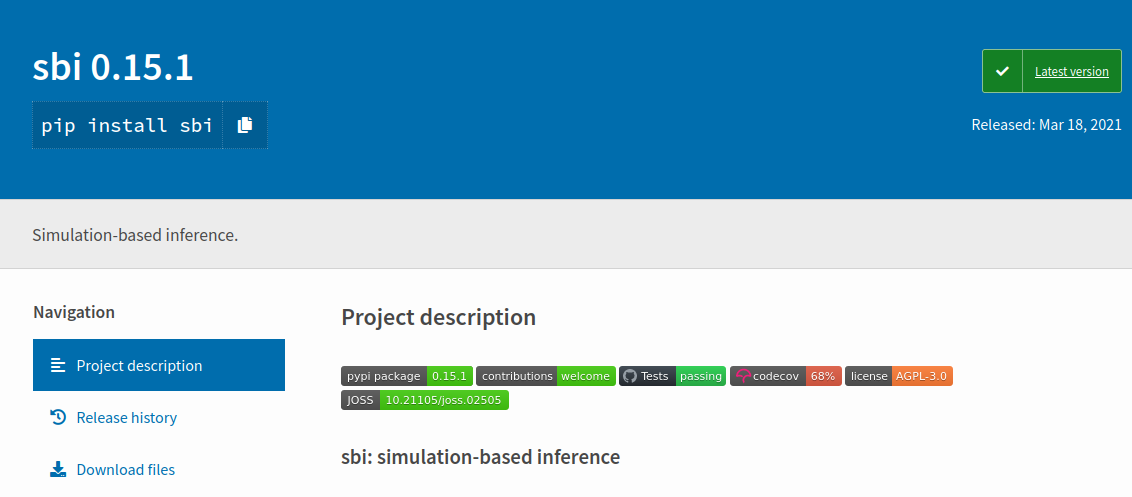
\includegraphics[width=.5\linewidth]{figures/sbipypi.png}
	\end{figure}
\end{itemize}
\end{frame} 


\begin{frame}
\frametitle{Questions for you}
\framesubtitle{Discussion}
\begin{itemize}
	\item Do you know a setting where SBI could be applied?
	\item What are downsides of SBI?
	\item Can't we just use a variational autoencoder?
\end{itemize}
\end{frame} 




\begin{frame}
\frametitle{References}
\framesubtitle{}
\bibliography{references}
\end{frame} 

\begin{frame}
\frametitle{}
\framesubtitle{}
\begin{itemize}
	\item Example (if there is time)
\end{itemize}
\end{frame} 






\end{document}


